\subsection{MNIST Data Set and Feature Selection}

We applied a perceptron model to classification of handwritten digits. MNIST is a standard data set with $28\times28$ pixel images of handwritten digits.
We selected the digits $0$ and $7$ and 500 training images for each class for our classification task, as they are reasonably diffenrent. To chose the right feature we plotted all regionprops in a scatter plot matrix,see figure \ref{perceptron:features} and selected solodity and eccentricity. To compare the batch and online version we used an equivalent number of maximal iterations. This means we took used the size of a batch times the maximum number of iterations in the batch case as the maximum number of iterations for the online algorithm. In our case we took $500000$ and $500$.

\begin{figure}
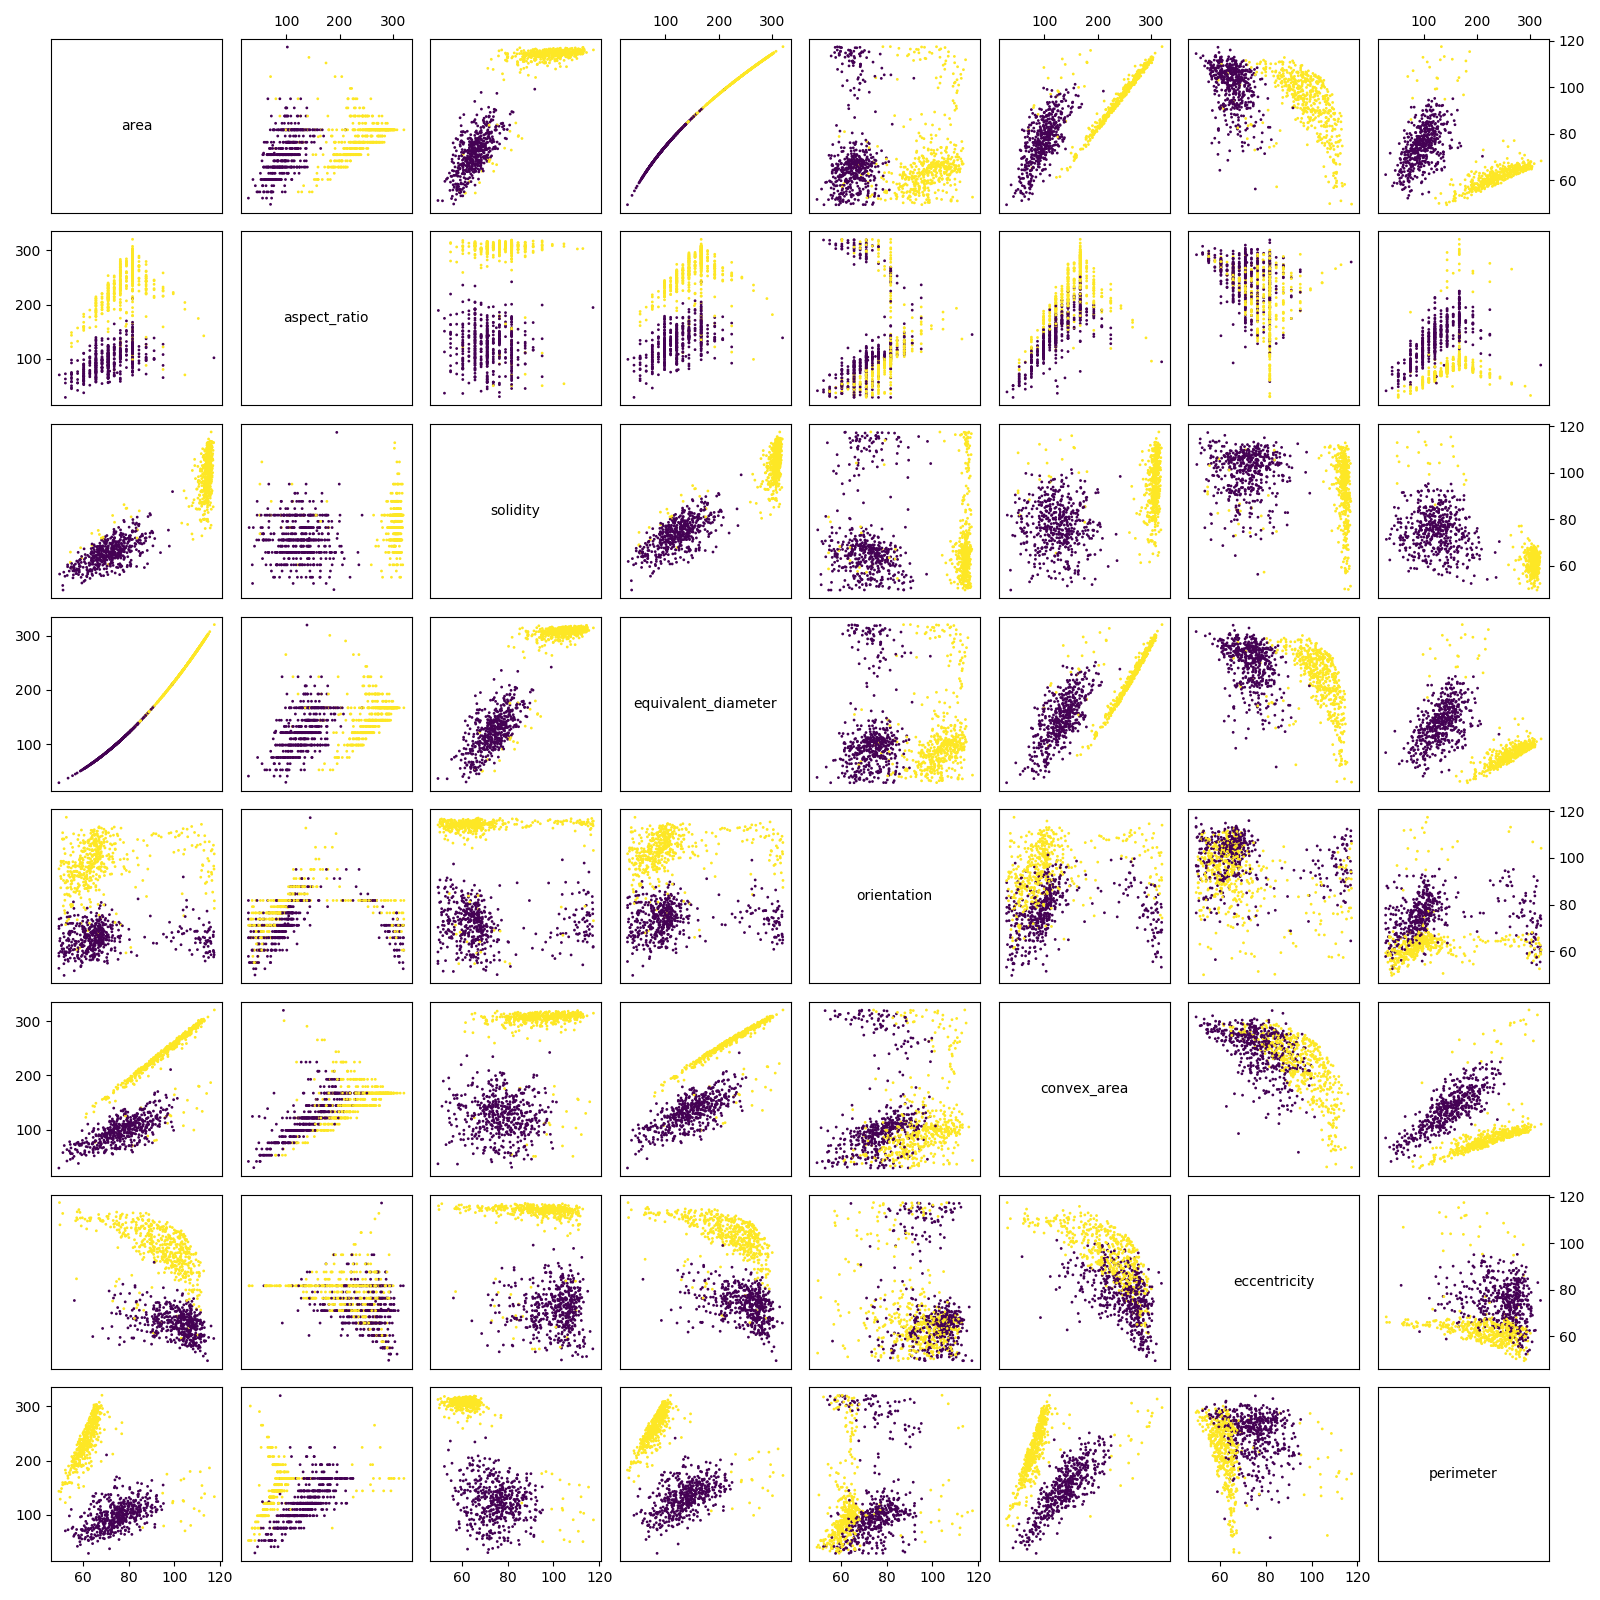
\includegraphics[width=\textwidth]{figures/scatter_matrix}
\caption{Scatter plot matrix of all region properties}
\label{perceptron:features}
\end{figure}

\subsubsection{Features without transform}

We used once the batch training algorithm and once the online training algorithm to classify the data directly from these to features. The connfusion matrix evaluated on a separate test set gives us following perfomance:

For the online training algorithm evaluated on the test set we got 385 correctly classified results of 400 test images. We got the following confusion matrix:

\begin{tabular}{ l | c | r }
\centering
  n=400 & classified as 1 & classified as 7 \\ \hline
  Digit 0 & 185 & 15 \\
  Digit 7 & 0 & 200 \\
\end{tabular}

For the batch training algorithm evaluated on the same test set we got 383 correctly classified results of 400 test images. We got the following confusion matrix:

\begin{tabular}{ l | c | r }
\centering
  n=400 & classified as 1 & classified as 7 \\ \hline
  Digit 0 & 187 & 13 \\
  Digit 7 & 4 & 200 \\
\end{tabular}

The corresponding decision boundries are shown in figure \ref{perceptron:decision:simple}. We see that the data is not linearly seperable, because there are yellow points inside the purple "cloud" In theory a perceptron is able to detect a linearly seperable set, because if the set is linearly seperable, then the algorithm is guaranteed to converge. Moreover we can bound the number of training steps from above. But as this bound depends on a separating hyperplane and the training set, we can not know beforehand how big this upper bound is.

\begin{figure}
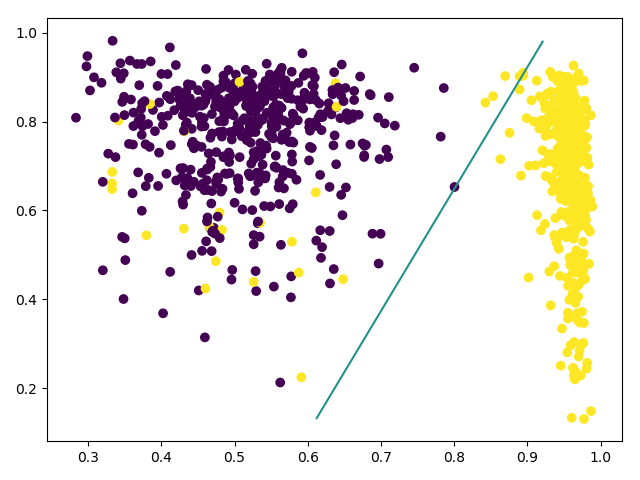
\includegraphics[width = 0.5\textwidth]{figures/decision_simple_online}
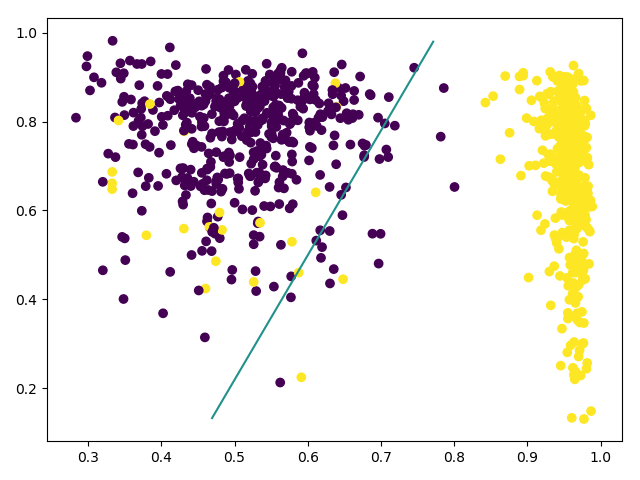
\includegraphics[width = 0.5\textwidth]{figures/decision_simple_batch}
\caption{On the decision boundry of the trained perceptron. On the left for the online algorithm on the right for the batch algorithm.}
\label{perceptron:decision:simple}
\end{figure}

\subsubsection{Classification with feature transform}

\subsubsection{Classification directly with image data}

